\documentclass[12pt]{article}

%useful packages
\usepackage{color,soul}
\usepackage[usenames,dvipsnames,svgnames,table]{xcolor}
\usepackage{amsmath,amsthm,amscd,amssymb,bm}
\usepackage{hyperref}
\hypersetup{
    colorlinks=true,
    linkcolor=JungleGreen
}
\usepackage[utf8]{inputenc}
\usepackage[top=2cm, bottom=3cm, left=2cm, right=2cm]{geometry}
\usepackage{pgfplots}
\usepackage{enumitem}
\usepgfplotslibrary{fillbetween}
\usetikzlibrary{patterns}
\usepackage{tcolorbox}
\usepackage{centernot}
\usepackage{mathtools}
\usepackage{xcolor}

%personal definitions and commands
\newcommand{\R}{\mathbb{R}} 
\newcommand{\E}{\mathbb{E}}
\newcommand{\V}{\mathbb{V}}
\newcommand{\C}{\mathbb{C}}
\newcommand{\Prob}{\mathbb{P}}
\newcommand{\e}{\epsilon}
\newcommand\numberthis{\addtocounter{equation}{1}\tag{\theequation}} %allows numbering of single equations in align* environment
\newcommand{\mtx}[1]{\ensuremath{\bm{\mathit{#1}}}}
\newcommand{\B}{\hat{\boldsymbol{\beta}}}
\newcommand{\Cov}{\mathbb{C}\text{ov}}
\newcommand{\N}{\mathcal{N}}



\title{ECON675 -- Assignment 3}
\author{Anirudh Yadav}
\setlength\parindent{0pt}
\begin{document}

\maketitle

\setcounter{tocdepth}{2}
\tableofcontents

\newpage

\section{Non-linear least squares}

\subsection{Identifiability}
This is a standard M-estimation problem. The parameter vector $\mtx{\beta}_0$ is assumed to solve the population problem
\begin{align*}
\mtx{\beta}_0 = \arg \min_{\beta \in \R^d} \E[(y_i - \mu(\mtx{x}_i'\mtx{\beta}))^2].
\end{align*}
For $\mtx{\beta}_0$ to be identified, it must be the \textit{unique} solution to the above population problem (i.e. the unique minimizer). In math, this means for all $\e>0$ and for some $\delta >0$:
\begin{align*}
\sup_{|| \beta - \beta_0 || > \e} M(\mtx{\beta}) \geq M(\mtx{\beta}_0) + \delta
\end{align*}
where $M(\mtx{\beta}) = \E[(y_i - \mu(\mtx{x}_i'\mtx{\beta}))^2]$. Of course $\mtx{\beta}_0$ can be written in closed form if $\mu(\cdot)$ is linear. In this case, we know that 
\begin{align*}
\mtx{\beta}_0= \E[\mtx{x}_i\mtx{x}_i']^{-1}\E[\mtx{x}_iy_i].
\end{align*}

\subsection{Asymptotic normality}
The M-estimator is asymptotically normal if:
\begin{enumerate}
\item $\hat{\mtx{\beta}} \to_p \mtx{\beta}_0$
\item $\mtx{\beta}_0 \in int(B)$ and $m(\mtx{x}_i,\mtx{\beta}) \equiv (y_i - \mu(\mtx{x}_i'\mtx{\beta}))^2$ is 3 times continuously differentiable.
\item $\Sigma_0 = \V[\frac{\partial}{\partial \beta} m(\mtx{x}_i; \beta_0)] < \infty$ and $H_0 = \E[\frac{\partial^2}{\partial \beta \partial \beta'} m(\mtx{x}_i; \beta_0)]$ is full rank (and therefore invertible).
\end{enumerate}
Now, the FOC for the M-estimation problem is
\begin{align}
0 &= \frac{1}{n} \sum_{i=1}^n (y_i-\mu(\mtx{x}_i'\mtx{\beta}))\dot{\mu}(\mtx{x}_i'\mtx{\beta}))\mtx{x}_i \label{eq:M1}
\end{align}
where $\dot \mu = \frac{\partial}{\partial \beta}  \mu (\mtx{x}_i'\mtx{\beta})$. So, we've converted the M-estimation problem into a Z-estimation problem. Then we can use the standard asymptotic normality result to arrive at a precise form of the asymptotic variance:
\begin{align*}
\sqrt{n}(\hat{\mtx{\beta}}-\mtx{\beta}_0) \to_d \N(0, H_0^{-1}\Sigma_0 H_0^{-1}).
\end{align*}
Now, taking the second derivative gives the Hessian
\begin{align*}
H_0 &= \E[\frac{\partial^2}{\partial \beta \partial \beta'} m(\mtx{x}_i; \beta_0)]\\
&=\E\left[-\dot{\mu}(\mtx{x}_i'\mtx{\beta}_0))\dot{\mu}(\mtx{x}_i'\mtx{\beta}_0))\mtx{x}_i\mtx{x}_i' + (y_i-\mu(\mtx{x}_i'\mtx{\beta}_0))\ddot{\mu}(\mtx{x}_i'\mtx{\beta}_0))\mtx{x}_i\mtx{x}_i'\right]\\
&=-\E[\dot{\mu}(\mtx{x}_i'\mtx{\beta}_0))^2\mtx{x}_i\mtx{x}_i']
\end{align*}
by LIE. And, the variance of the score is
\begin{align*}
\Sigma_0 &= \V[\frac{\partial}{\partial \beta} m(\mtx{x}_i; \beta_0)] \\
&=\E\left[(y_i-\mu(\mtx{x}_i'\mtx{\beta}_0))^2\dot{\mu}(\mtx{x}_i'\mtx{\beta}_0))^2\mtx{x}_i\mtx{x}_i'\right]\\
&=\E[\sigma^2(\mtx{x}_i)\dot{\mu}(\mtx{x}_i'\mtx{\beta}_0))^2\mtx{x}_i\mtx{x}_i']
\end{align*}
again by LIE. Then we have the asymptotic variance
\begin{align*}
\mtx{V}_0 = H_0^{-1}\Sigma_0 H_0^{-1}.
\end{align*}

\subsection{Variance estimator under heteroskedasticity}
Under heteroskedasticity we can use the sandwich variance estimator
\begin{align*}
\widehat{\mtx{V}}_{HC} &= \hat{H}^{-1}\hat \Sigma \hat{H}^{-1},
\end{align*}
where
\begin{align*}
\hat{H} &= \frac{1}{n} \sum_{i=1}^n \dot{\mu}(\mtx{x}_i'\hat{\mtx{\beta}}))^2\mtx{x}_i\mtx{x}_i'\\
\hat \Sigma &= \frac{1}{n} \sum_{i=1}^n \hat{e}^2_i\dot{\mu}(\mtx{x}_i'\hat{\mtx{\beta}}))^2\mtx{x}_i\mtx{x}_i'\\
\end{align*}
Now, to get an asymptotically valid CI for $|| \mtx{\beta}_0 ||^2$ we need to use the Delta Method. First, note that:
\begin{align*}
|| \mtx{\beta}_0 ||^2 &= \mtx{\beta}_0 ' \mtx{\beta}_0 \\
\implies \frac{\partial}{\partial \beta}|| \mtx{\beta}_0 ||^2 & = 2\mtx{\beta}_0
\end{align*}
Then, using the Delta Method
\begin{align*}
\sqrt{n}(||\hat{\mtx{\beta}}||^2-||\mtx{\beta}_0||^2) &\to_d 2\mtx{\beta}_0 \N(0,\mtx{V}_0)\\ 
&= \N(0,4 \mtx{\beta}_0'\mtx{V}_0 \mtx{\beta}_0)
\end{align*}
Thus, an asymptotically valid 95\% CI for $|| \mtx{\beta}_0 ||^2$ is
\begin{align*}
CI_{95} = \left[\hat{\mtx{\beta}} - 1.96 \sqrt{\frac{4\hat{\mtx{\beta}}'\widehat{\mtx{V}}_{HC}\hat{\mtx{\beta}}}{n}},\hat{\mtx{\beta}} + 1.96 \sqrt{\frac{4\hat{\mtx{\beta}}'\widehat{\mtx{V}}_{HC}\hat{\mtx{\beta}}}{n}}\right]
\end{align*}

\subsection{Variance estimator under homoskedasticity}
Using the above results, under homoskedasticity, the asymptotic variance collapses to
\begin{align*}
\mtx{V}_0 &= \E[\dot{\mu}(\mtx{x}_i'\mtx{\beta}_0))^2\mtx{x}_i\mtx{x}_i']^{-1} \sigma^2 \E[\dot{\mu}(\mtx{x}_i'\mtx{\beta}))^2\mtx{x}_i\mtx{x}_i'] \E[\dot{\mu}(\mtx{x}_i'\mtx{\beta}_0))^2\mtx{x}_i\mtx{x}_i']^{-1}\\
&=\sigma^2\E[\dot{\mu}(\mtx{x}_i'\mtx{\beta}_0))^2\mtx{x}_i\mtx{x}_i']^{-1}
\end{align*}
The variance estimator is now takes a simpler form
\begin{align*}
\widehat{\mtx{V}}_{HO} &= \hat{\sigma}^2 \hat{H}^{-1}
\end{align*}
where $\hat{H}$ is the same as above and
\begin{align*}
\hat{\sigma}^2 &= \frac{1}{n-d} \sum_{i=1}^n (y_i-\mu(\mtx{x}_i'\hat{\mtx{\beta}}))^2
\end{align*}
Then, as above, the asymptotically valid 95\% CI for $|| \mtx{\beta}_0 ||^2$ is
\begin{align*}
CI_{95} = \left[\hat{\mtx{\beta}} - 1.96 \sqrt{\frac{4\hat{\mtx{\beta}}'\widehat{\mtx{V}}_{HO}\hat{\mtx{\beta}}}{n}},\hat{\mtx{\beta}} + 1.96 \sqrt{\frac{4\hat{\mtx{\beta}}'\widehat{\mtx{V}}_{HO}\hat{\mtx{\beta}}}{n}}\right].
\end{align*}

\subsection{MLE}
Given the assumption of a normal DGP we have the conditional density
\begin{align*}
f(y_i|\mtx{x}_i) = \frac{1}{\sqrt{2\pi\sigma^2}}\exp\Big(-\frac{1}{2\sigma^2}(y_i - \mu(\mtx{x}'_i\mtx{\beta}_0))^2\Big).
\end{align*}
Then, the sample log-likelihood function is
\begin{align*}
\ell(\mtx{\beta}, \sigma^2; \mtx{X}) &= n \log\Big(\frac{1}{\sqrt{2\pi\sigma^2}}\Big) -\frac{1}{2\sigma^2}\sum_{i=1}^n(y_i - \mu(\mtx{x}'_i\mtx{\beta}))^2
\end{align*}
Dividing by $n$ gives
\begin{align*}
\ell(\mtx{\beta},\sigma^2; \mtx{X}) &= \log\Big(\frac{1}{\sqrt{2\pi\sigma^2}}\Big) -\frac{1}{n2\sigma^2}\sum_{i=1}^n(y_i - \mu(\mtx{x}'_i\mtx{\beta}))^2
\end{align*}
The FOC wrt $\mtx{\beta}$ is
\begin{align*}
0 &= \frac{1}{n\sigma^2} \sum_{i=1}^n (y_i-\mu(\mtx{x}_i'\mtx{\beta}))\dot{\mu}(\mtx{x}_i'\mtx{\beta}))\mtx{x}_i,
\end{align*}
which is equivalent to the FOC for the M-estimation problem (\ref{eq:M1}) (since $\sigma^2$ just scales the FOC, it does not affect the solution). Thus,
\begin{align*}
\hat{\mtx{\beta}}_{MLE} =\hat{\mtx{\beta}}_{M.est}.
\end{align*}
Now, the FOC of the log-likelihood wrt $\sigma^2$ is
\begin{align*}
0 = -\frac{1}{2}(2\pi\sigma^2)^{-1}2\pi + \frac{1}{2n}(\sigma^2)^{-2} \sum_{i=1}^n (y_i-\mu(\mtx{x}_i'\hat{\mtx{\beta}}))^2
\end{align*}
Solving for $\sigma^2$ gives the MLE:
\begin{align*}
\hat \sigma^2_{ML} = \frac{1}{n} \sum_{i=1}^n (y_i-\mu(\mtx{x}_i'\hat{\mtx{\beta}}))^2,
\end{align*}
which is not the same as the estimator proposed in [4], since it does not adjust for the number of regressors.

\subsection{When the link function is unknown}
Suppose the link function is unknown, and consider two pairs of true parameters, $(\mu_1,{\mtx{\beta}}_1)$ and $(\mu_2,{\mtx{\beta}}_2)$ where $\mu_2(u)$ = $\mu_1(u/c)$ and ${\mtx{\beta}}_2= c{\mtx{\beta}}_1$ for some $c\neq 0$. Then the parameters are clearly different, but $\mu_1(\mtx{x}'_i\mtx{\beta}_1)=\mu_2(\mtx{x}'_i\mtx{\beta}_2)$. 

\subsection{Logistic link function}
The link function is
\begin{align*}
\mu(\mtx{x}'_i\mtx{\beta}_0) &=\E[y_i|\mtx{x}_i]\\
&= \E[\bm{1}(\mtx{x}'_i\mtx{\beta}_0 \geq \e_i) |\mtx{x}_i ]\\
&=\Pr[\mtx{x}'_i\mtx{\beta}_0 \geq \e_i |\mtx{x}_i ]\\
&= F(\mtx{x}'_i\mtx{\beta}_0)\\
&= \frac{1}{1+ \exp(-\mtx{x}'_i\mtx{\beta}_0)}, \text{ if } s_0 = 1.
\end{align*}
The conditional variance of $y_i$ is
\begin{align*}
\sigma^2(\mtx{x}_i)  \V[y_i | \mtx{x}_i]\\
\end{align*}
Now, note that $y_i|\mtx{x}_i$ is a Bernoulli random variable, with $\Pr[y_i=1 |\mtx{x}_i] = F(\mtx{x}'_i\mtx{\beta}_0)$. Then
\begin{align*}
\sigma^2(\mtx{x}_i)  &= F(\mtx{x}'_i\mtx{\beta}_0)(1-F(\mtx{x}'_i\mtx{\beta}_0))\\
&= \mu(\mtx{x}'_i\mtx{\beta}_0)(1-\mu(\mtx{x}'_i\mtx{\beta}_0))
\end{align*}

To derive an expression for the asymptotic variance, first note that for the logistic cdf: $\dot \mu(u) = (1-\mu(u))\mu(u)$. Then, the asymptotic variance is 
\begin{align*}
\mtx{V}_0 &= H_0^{-1}\Sigma_0 H_0^{-1}.
\end{align*}
where
\begin{align*}
H_0 = \E[(1-\mu(\mtx{x}'_i\mtx{\beta}_0))^2 \mu(\mtx{x}'_i\mtx{\beta}_0)^2 \mtx{x}_i\mtx{x}_i']
\end{align*}
and
\begin{align*}
\Sigma_0 =  \E[(1-\mu(\mtx{x}'_i\mtx{\beta}_0))^3 \mu(\mtx{x}'_i\mtx{\beta}_0)^3 \mtx{x}_i\mtx{x}_i']
\end{align*}

\subsection{Logistic link function, MLE}
MLE gives the same point estimator as NLS (i.e. they have the same FOC; we did this in 672), but MLE is asymptotically efficient, so $\mtx{V}_0^{ML} \leq \mtx{V}_0^{NLS}$.

\subsection{Some data work}

\textbf{(a)} I estimated the logistic model with robust (HC1) standard errors in both \verb|R| and \verb|Stata|. The results from \verb|R| are presented in Table 1. The standard errors from \verb|Stata| are very slightly different, but I'm not sure why.

\begin{table}[!htpb]
\centering
\caption{\textbf{Logistic Regression Estimates for $s=1-$\texttt{dmissing}}}
\begin{tabular}{lrrrrrr}
  \hline
 & Coef. & Std. Err. & t-stat & p-val & CI.lower & CI.upper \\ 
  \hline
Const. & 1.755 & 0.335 & 5.245 & 0.000 & 1.099 & 2.411 \\ 
  S\_age & 1.333 & 0.123 & 10.826 & 0.000 & 1.092 & 1.575 \\ 
  S\_HHpeople & -0.067 & 0.023 & -2.871 & 0.004 & -0.112 & -0.021 \\ 
  $\log(\text{inc}+1)$ & -0.119 & 0.044 & -2.707 & 0.007 & -0.205 & -0.033 \\ 
   \hline
\end{tabular}
\end{table}

\textbf{(b)} Table 2 presents the 95\% confidence interval and p-values for each coefficient derived from 999 bootstrap replications of the t-statistic: $t^*=({\beta^*}-\hat{\beta}_{obs})/se^*$. The statistics are very similar to those in Table 1, which rely on large sample approximations. \\

The idea for computing bootstrapped CIs is simple: for each bootstrap replication, compute $t^*$ for each coefficient; this gives an empirical distribution for $t^*$; then extract the desired quantiles from the empirical distribution, and compute the confidence intervals as
\begin{align*}
CI^{boot}_{95}(\beta) = \left[ \hat{\beta}_{obs} +q^*_{0.025}\times \hat{se}_{obs},\text{ } \hat{\beta}_{obs} +q^*_{0.975}\times \hat{se}_{obs} \right]
\end{align*}
I computed the bootstrapped p-values as 
\begin{align*}
p^{boot} = \frac{1}{M}\sum_{i=1}^M \bm{1}[t^* \geq t_{obs}]
\end{align*}
where $M$ is the number of bootstrap replications.

\begin{table}[!htpb]
\centering
\caption{\textbf{Bootstrap Statistics for the Logistic Model of $s=1-$\texttt{dmissing}}}
\begin{tabular}{lrrrr}
  \hline
 & Coef. & CI.lower & CI.upper & p-val \\ 
  \hline
Const. & 1.755 & 1.157 & 2.471 & 0.000 \\ 
  S\_age & 1.333 & 1.142 & 1.609 & 0.000 \\ 
  S\_HHpeople & -0.067 & -0.112 & -0.020 & 0.001 \\ 
  $\log(\text{inc}+1)$  & -0.119 & -0.216 & -0.042 & 0.001 \\ 
   \hline
\end{tabular}
\end{table}

\textbf{(c)} I plot the kernel density estimate of the predicted probabilities of reporting data, $\hat{\mu}(\mtx{x}'_i\hat{\mtx{\beta}})$, using an Epanechnikov kernel with \verb|R|'s unbiased cross-validation bandwidth.

\begin{figure}[!htpb]
    \centering
    
        %\centering
        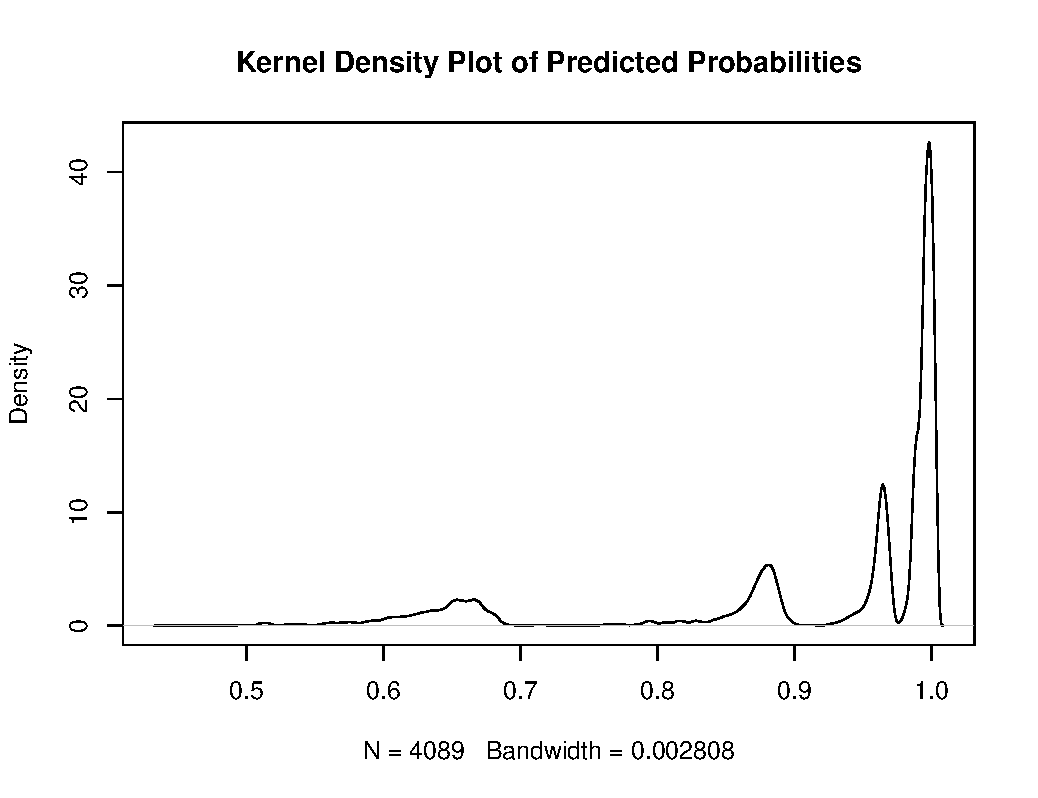
\includegraphics[width=0.7\textwidth]{kdens.pdf}

\end{figure}

\newpage


\section{Semiparametric GMM with missing data}

\subsection{An optimal instrument}
We have the conditional moment condition:
\begin{align*}
\E[m(y_i^*, t_i, \mtx{x}_i; \mtx{\beta}_0)|t_i,\mtx{x}_i] =0
\end{align*}
By LIE
\begin{align*}
\E\big[\mtx{g}(t_i,\mtx{x}_i)\E[m(y_i^*, t_i, \mtx{x}_i; \mtx{\beta}_0)|t_i,\mtx{x}_i]\big] =0
\end{align*}
for any $\mtx{g}(\cdot)$. Thus,
\begin{align*}
\E\big[\E[\mtx{g}(t_i,\mtx{x}_i)m(y_i^*, t_i, \mtx{x}_i; \mtx{\beta}_0)|t_i,\mtx{x}_i]\big] &=0\\
\implies \E[\mtx{g}(t_i,\mtx{x}_i)m(y_i^*, t_i, \mtx{x}_i; \mtx{\beta}_0)] &=0
\end{align*}
Now, we want to find the optimal $\mtx{g}$ that minimizes $\text{AsyVar}(\hat{\mtx{\beta}})$; call it $\mtx{g}_0$. Let $\mtx{z}_i=(t_i,\mtx{x}_i)$, $\mtx{w}_i = (y_i^*,t_i,\mtx{x}_i)$. The GMM estimator is
\begin{align*}
\hat{\mtx{\beta}} &= \arg \min_{\beta \in \R^d}\left(\frac{1}{n}\sum_{i=1}^n \mtx{g}(\mtx{z}_i)m(\mtx{w}_i,\mtx{\beta})\right)'\mtx{W} \left(\frac{1}{n}\sum_{i=1}^n \mtx{g}(\mtx{z}_i)m(\mtx{w}_i,\mtx{\beta})\right)
\end{align*}
The FOC wrt $\mtx{\beta}$ is
\begin{align*}
0 &= \left(\frac{1}{n}\sum_{i=1}^n \frac{\partial}{\partial \beta}\mtx{g}(\mtx{z}_i)m(\mtx{w}_i,\mtx{\beta})\right)'\mtx{W}\left(\frac{1}{n}\sum_{i=1}^n \mtx{g}(\mtx{z}_i)m(\mtx{w}_i,\mtx{\beta})\right)
\end{align*}
We can write the FOC plugging in $\hat{\mtx{\beta}}$:
\begin{align*}
0 &= \left(\frac{1}{n}\sum_{i=1}^n \frac{\partial}{\partial \beta}\mtx{g}(\mtx{z}_i)m(\mtx{w}_i,\hat{\mtx{\beta}})\right)'\mtx{W}\left(\frac{1}{n}\sum_{i=1}^n \mtx{g}(\mtx{z}_i)m(\mtx{w}_i,\hat{\mtx{\beta}})\right).
\end{align*}
Then, if we take a mean value Taylor expansion of the last term in parentheses around the true parameter $\mtx{\beta}_0$ and rearrange in the usual way, we get
\begin{align*}
\sqrt{n}(\hat{\mtx{\beta}} - \mtx{\beta}_0) = -\left[\mtx{G}_n(\hat{\mtx{\beta}})'\mtx{W}\mtx{G}_n(\tilde{\mtx{\beta}})\right]^{-1}\mtx{G}_n(\hat{\mtx{\beta}})'\mtx{W}\left( \frac{1}{\sqrt{n}} \sum_{i=1}^n \mtx{g}(\mtx{z}_i)m(\mtx{w}_i,\mtx{\beta}_0)\right)
\end{align*}
where
\begin{align*}
\mtx{G}_n({\mtx{\beta}}) = \frac{1}{n}\sum_{i=1}^n \frac{\partial}{\partial \beta}\mtx{g}(\mtx{z}_i)m(\mtx{w}_i,\mtx{\beta})
\end{align*}
Now we just need to let things converge via LLN and CLT to get
\begin{align*}
\sqrt{n}(\hat{\mtx{\beta}} - \mtx{\beta}_0)  \to_d \N\left(0, \left[\mtx{G}({\mtx{\beta}_0})'\mtx{W}\mtx{G}({\mtx{\beta}_0})\right]^{-1}\mtx{G}({\mtx{\beta}_0})'\mtx{W}\V[\mtx{g}(\mtx{z}_i)m(\mtx{w}_i,\mtx{\beta}_0)] \mtx{W}\mtx{G}({\mtx{\beta}_0} \left[\mtx{G}({\mtx{\beta}_0})'\mtx{W}\mtx{G}({\mtx{\beta}_0})\right]^{-1}\right)
\end{align*}
Then with the optimal weight matrix $\mtx{W} = \V[\mtx{g}(\mtx{z}_i)m(\mtx{w}_i,\mtx{\beta}_0)]^{-1}$ the asymptotic variance collapses to
\begin{align*}
\mtx{V}_0 = \left[\mtx{G}({\mtx{\beta}_0})'\V[\mtx{g}(\mtx{z}_i)m(\mtx{w}_i,\mtx{\beta}_0)]^{-1}\mtx{G}({\mtx{\beta}_0})\right]^{-1}
\end{align*}
And, as shown in class, this leads to the optimal instrument
\begin{align*}
\mtx{g}_0(\mtx{z}_i) =\E\left[\frac{\partial}{\partial \beta}m(\mtx{w}_i,\mtx{\beta})| \mtx{z}_i\right] \V[m(\mtx{w}_i,\mtx{\beta}_0)|\mtx{z}_i]^{-1}
\end{align*}
Now, in the given case, since $y_i$ is Bernoulli we know that
\begin{align*}
\V[m(\mtx{w}_i,\mtx{\beta}_0)|\mtx{z}_i] = F(t_i\theta_0 +\mtx{x}_i'\mtx{\gamma}_0)[1-F(t_i\theta_0 +\mtx{x}_i'\mtx{\gamma}_0)]
\end{align*}
And
\begin{align*}
\E\left[\frac{\partial}{\partial \beta}m(\mtx{w}_i,\mtx{\beta})| \mtx{z}_i\right] = f(t_i\theta_0 +\mtx{x}_i'\mtx{\gamma}_0)[t_i , \mtx{x}_i]',
\end{align*}
which gives the desired result. When $F(\cdot)$ is the logistic cdf we know that
\begin{align*}
f(u) = F(u)[1-F(u)],
\end{align*}
so that
\begin{align*}
\mtx{g}_0(t_i,\mtx{x}_i) = [t_i , \mtx{x}_i]'.
\end{align*}

\subsection{Missing completely at random}
\textbf{(a)}The optimal unconditional moment condition is:
\begin{align*}
\E[\mtx{g}_0(t_i,\mtx{x}_i)m(y_i^*, t_i, \mtx{x}_i; \mtx{\beta}_0)] &=0
\end{align*}
Now, $y_i = s_iy_i^*$. Thus,
\begin{align*}
\E[\mtx{g}_0(t_i,\mtx{x}_i)m(y_i, t_i, \mtx{x}_i; \mtx{\beta}_0)|s_i = 1] &=\E[\mtx{g}_0(t_i,\mtx{x}_i)m(y_i^*, t_i, \mtx{x}_i; \mtx{\beta}_0)|s_i = 1] 
\end{align*}
And, with the MCAR assumption, the above moment condition is identical to the optimal one. Accordingly, a feasible estimator is simply
\begin{align*}
\hat{\mtx{\beta}}_{\texttt{MCAR,feasible}}= \arg \min_{\theta, \gamma} \frac{1}{n} \sum_{i=1}^n [s_i \mtx{g}_0(t_i,\mtx{x}_i)(y_i-F(t_i \theta+\mtx{x}_i'\mtx{\gamma}))].
\end{align*}

\textbf{(b)}
I report the the results from using the feasible estimator below.

\begin{table}[ht]
\centering
\begin{tabular}{lrrrrrr}
  \hline
 & Estimate & Std.Error & t & p-value & CI.lower & CI.upper \\ 
  \hline
dpisofirme & -0.325 & 0.105 & -3.106 & 0.032 & -0.518 & -0.167 \\ 
  S\_age & -0.226 & 0.024 & -9.326 & 0.000 & -0.275 & -0.177 \\ 
  S\_HHpeople & 0.027 & 0.018 & 1.563 & 0.140 & -0.006 & 0.061 \\ 
  log\_inc & 0.023 & 0.017 & 1.341 & 0.184 & -0.010 & 0.060 \\ 
   \hline
\end{tabular}
\end{table}


\subsection{Missing at random}
Start with the optimal moment condition
\begin{align*}
\E[\mtx{g}_0(t_i,\mtx{x}_i)m(y_i^*, t_i, \mtx{x}_i; \mtx{\beta}_0)] &=0.
\end{align*}
Since $y_i=s_i*y_i^*$ and $s_i \perp y_i^*|(t_i,x_i)$,
\begin{align*}
\E[s_i m(y_i^*, t_i, \mtx{x}_i; \mtx{\beta}_0)|t_i,x_i]&=\E[\mtx{g}(t_i,\mtx{x}_i)m(y_i^*, t_i, \mtx{x}_i; \mtx{\beta}_0)]
\end{align*}
Thus, $\E[s_i m(y_i^*,t_i,x_i; \beta_0)|t_i,x_i]=0$ is equivalent to the optimal unconditional moment restriction.\\

\textbf{(b)}\\

\textbf{(c)}\\

\textbf{(d)}




\newpage

\section{When bootstrap fails}

\subsection{Nonparametric bootstrap fail}
I plot the empirical distribution of the bootstrap statistic, $n(\max\{x_i\} - \max\{x_i^*\})$, below. Clearly, the empirical distribution does not coincide with the theoretical Exponential (1) distribution.

\begin{figure}[!htpb]
    \centering
    
        %\centering
        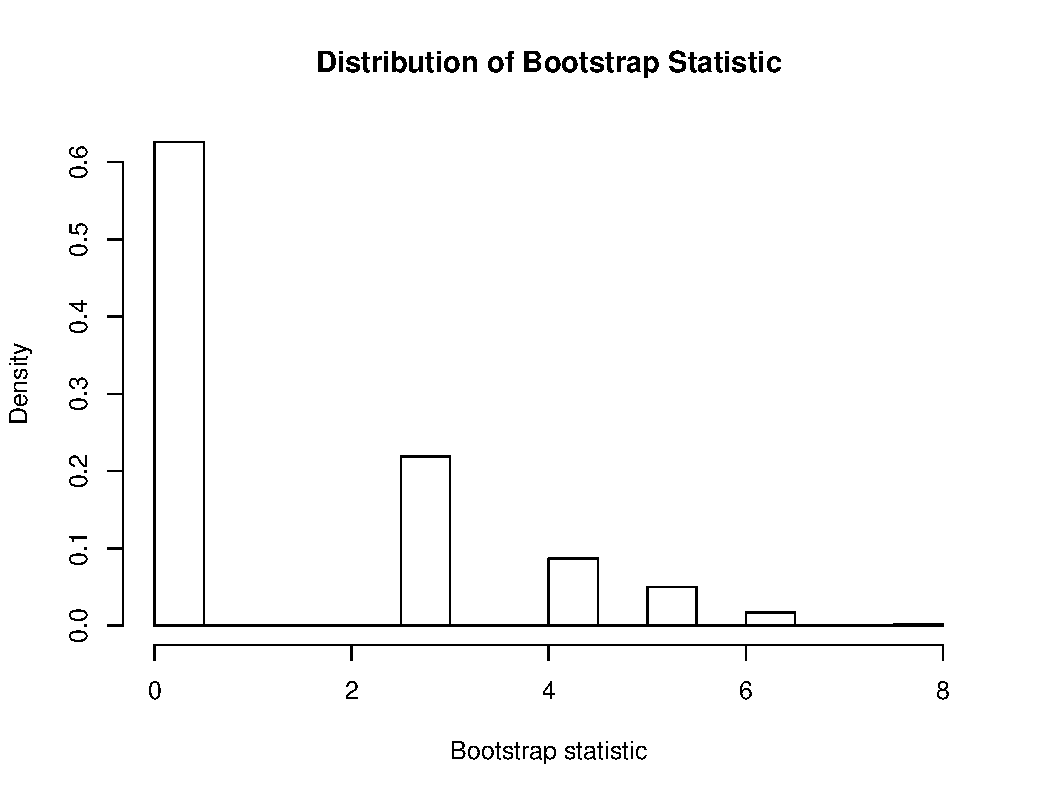
\includegraphics[width=0.7\textwidth]{freq.pdf}

\end{figure}

\subsection{Parametric bootstrap to the rescue}
Now, consider the parametric bootstrap statistic, $t^*_{\texttt{P}}= n(\max\{x_i\} - \max\{x_i^*\})$, where $$x_i^* \sim_{iid} \texttt{Uniform}[0,\max\{x_i\}].$$ I plot the empirical distribution of $t^*_{\texttt{P}}$ below. Now, the empirical distribution \textit{does} seem to coincide with the theoretical Exponential (1) distribution.

\begin{figure}[!htpb]
    \centering
    
        %\centering
        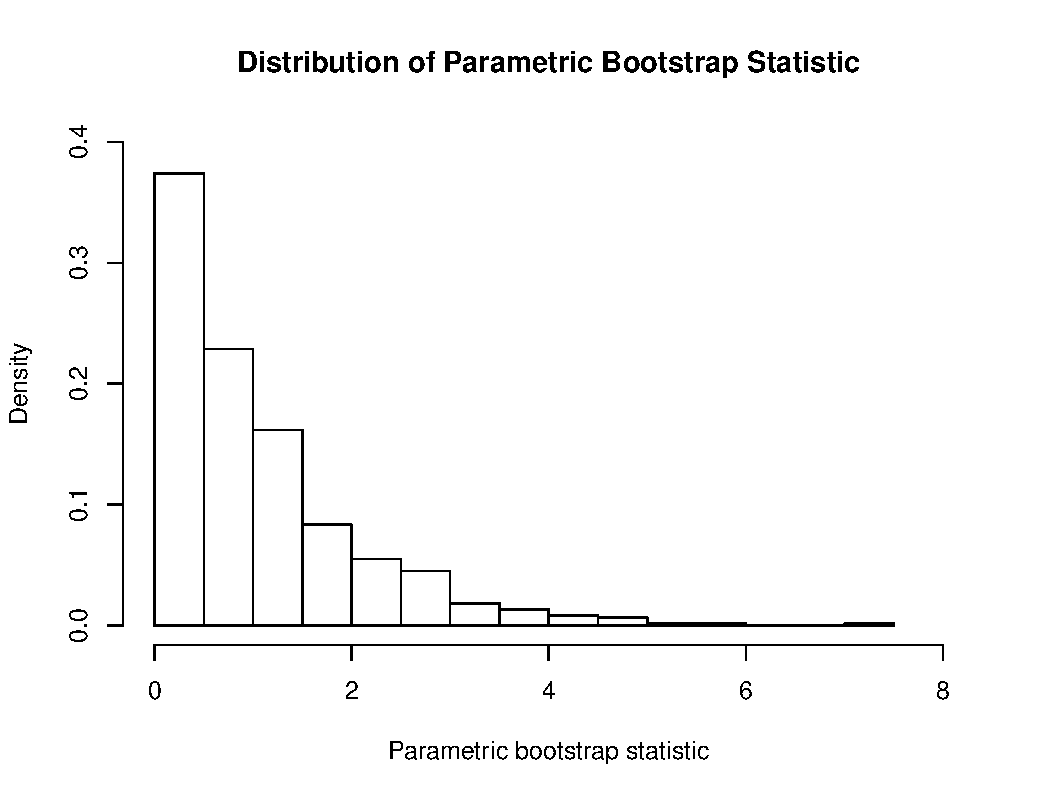
\includegraphics[width=0.7\textwidth]{freq2.pdf}

\end{figure}

\subsection{Intuition} In the nonparametric case, the bootstrap statistic has a mass point at zero since $\Pr[\max\{x_i\} = \max\{x_i^*\}]$ converges to 1. However, the parametric bootstrap corrects for this ``bias'': in this case $\Pr[\max\{x_i\} = \max\{x_i^*\}] = 0$, since $x_i^* \sim_{iid} \texttt{Uniform}[0,\max\{x_i\}].$

\newpage

\section{Appendix}

\subsection{\texttt{R} code}
\subsection{\texttt{STATA} code}


\end{document}
